\documentclass[../main.tex]{subfiles}

\begin{document}

\subsection{Estribos en puentes}

Los estribos son los apoyos extremos de los puentes, destinados a establecer
continiuidad entre la estructura y la carretera. Son dispuestas sobre un
relleno de acceso, y seben ser capaces de soportar las reacciones trasmitidas
por la estructura, soportar empujes por los rellenos de tierras de su trasdós
y servir de protección.

En sí, se componen de un muro frontal que recibe la carga del tablero, y muros
laterales que tienen como función asegurar el material del terraplen.

Podemos distinguir los siguientes tipos de estribos:


\subsubsection{Estribos de tramos rectos}

Cuando los estribos estan emplazados en 
tierra firme es frecuente que el muro frotnal y los laterales vayan cimentados
a la misma cota, y se busca una reducción en la obra de fábrica de los muros 
laterales, que se hace disponiendo de aletas abiertas cuya coronación se 
adapta a la línea de intersección en el terraplén.
El muro frontal debe ser calculado para el empuje de tierras y reacciones del
tablero.

Un ejemplo de lo dicho se encuentra en la siguiente figura:

\begin{figure}[ht]
  \centering
  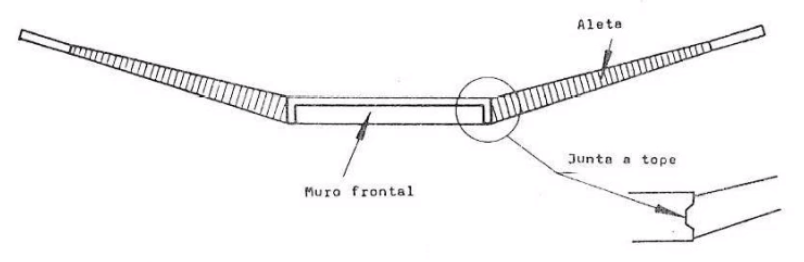
\includegraphics[width=0.8\textwidth]{../images/20210426/estribo_recto}
  \caption{Estribos con muro de frente y alas}
  \label{fig:estribo_recto}
\end{figure}

Estos estribos necesitan de una junta en el borde, que permite resolver la 
unión con un murete y la losa de transición que lo une al terraplen.

% COMPLETAR

\subsection{Socavación}

Las cimentaciones de las pilas y estribos requieren resistir los esfuerzos
dados por las socavaciones producidas por el régimen de crecidas de los cauces.
Podemos distinguir distintos tipos de socavaciones.

\subsubsection{Socavación general del lecho}

Se da cuando un lecho en una crecida aumenta la velocidad del agua y la capacidad
de arrastre, orginandose remoción de materiales del fondo. Luego de la 
crecida se dan sedimentaciones que esconden la socavación que se da en la cresta
de la crecida, pero es necesario tener en cuenta esta máxima socavación
\textit{durante} la crecida.

En general, los ciclos anuales forman socavaciones permanentes en los cursos
altos, estables en los medios y sedimentaciones en las zonas inferiores de los
ríos que han alcanzado su régimen de equilibrio. Este equilibrio puede alterarse
por el retiro de gravas y arenas en algun punto del cauce para la obtención
de materiales de construcción.

Por \textit{socavación general} se entiende como el descenso que tiene lugar
en el fondo del río al producirse una avenida y es debida al aumento de la
capacidad de arrastre al aumentar la velocidad del agua. La posibilidad de arrastre
de los materiales de fondo dependerá de la relación entre la velocidad media
del agua y la velocidad requerida para arrastrar las partículas que lo constituyen.

\begin{figure}[ht]
  \centering
  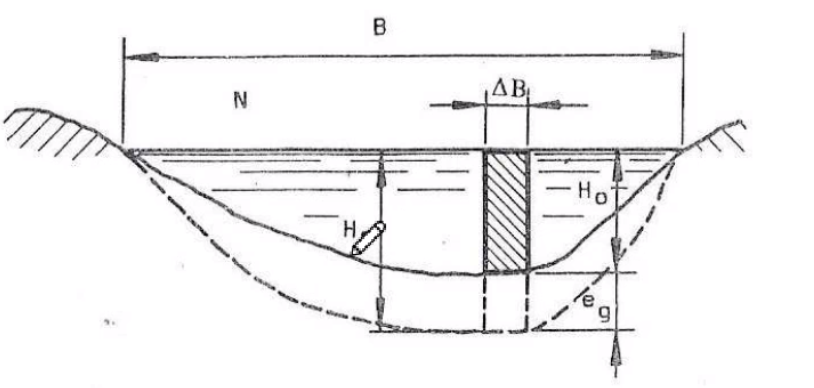
\includegraphics[width=0.8\textwidth]{../images/20210426/socavacion}
  \caption{socavacion}
  \label{fig:socavacion}
\end{figure}

La profundida puede ser determinada mediante dos tipos de métodos

\begin{description}
  \item[Método de cálculo empírico] se estiman las profundidades de socavación
    según empirismos que relacionaban la profunidad socavada con la altura de
    elevación de la lamina libre en la crecida. No son muy confiables.

  \item[Método teórico-práctico] busca determinar el descenso general del fondo
    del río. Considera una caudal $Q$ que siempre permanece constante y que la 
    velocidad media $V_o$ es la velocidad real del agua y donde $V_e$ es una 
    velocidad erosiva necesaria para el arrastre de partículas. Entonces, siempre
    que $V_o \geq V_e$, se producesirá erosión. Esto generará que aumente la
    sección del cauce, lo que hará que la veloicdad disminuya (ya que $Q=\text{cte}$),
    por lo que en algún momento se dará que $V_e \geq V_o$.


\end{description}


\end{document}
